% (fold)
% Template: LaTeX file for ICMC 2010 papers, with hyper-references
%
% derived from the DAFx-06 templates
% derived from the ICMC 2009 templates by Steve Beck
%
% 1) Please compile using latex or pdflatex.
% 2) Please use figures in vectorial format (.pdf); .png or .jpg are working otherwise 
% 3) Please use the "papertitle" and "pdfauthor" commands defined below

%------------------------------------------------------------------------------------------
\documentclass[twoside,10pt]{article}
\usepackage{icmc2010,amssymb,amsmath} 
%\setcounter{page}{1}

\usepackage{mathptmx} 

%____________________________________________________________
%  !  !  !  !  !  !  !  !  !  !  !  ! user defined variables  !  !  !  !  !  !  !  !  !  !  !  !  !  !
%==== set the title ====
\def\papertitle{A Flexible and Dynamic C++ Framework and Library for Digital Audio Signal Processing}
%\def\papertitle{}	%-- should be empty for the submission anyway!

%==== 1st submission: author name and affiliation are empty for anonymous submission ====
\def\paperauthorA{} 
\affiliation{}{}


%==== final submission: author name and affiliation ====
%---- uncomment 1 to 4 lines, for 1 to 4 authors
\def\paperauthorA{First Author}
\def\paperauthorB{Second Author}
\def\paperauthorC{Third Author}
\def\paperauthorD{Fourth Author}

%%---- set correspnding affiliation data for...
%%-- 1 author
%\affiliation{\paperauthorA}
%  {School\\ Department, City, Country \\ {\tt \href{mailto:email@domain.icmc}{email@domain.icmc}}}

%%-- 2 authors with same affiliation
%\affiliation{\paperauthorA, \paperauthorB}
%  {School\\ Department, City, Country \\ {\tt \href{mailto:email@domain.icmc}{email@domain.icmc}}}

%-- 2 authors with different affiliations
%\twoaffiliations{\paperauthorA}{School\\ Department}
%  {\paperauthorB}{Company\\ Address}

%%-- 3 authors with different affiliations
%\threeaffiliations{\paperauthorA}{School A\\ Department X}
%  {\paperauthorB}{Company\\ Address}
%  {\paperauthorC}{School B\\ Department Y}

%%-- 4 authors with different affiliations
%\fouraffiliations{\paperauthorA}{School A\\ Department X}
%  {\paperauthorB}{Company\\ Address}
%  {\paperauthorC}{School B\\ Department Y}
%  {\paperauthorD}{School C\\ Department Z}

%  ^  ^  ^  ^  ^  ^  ^  ^  ^  ^ user defined variables  ^  ^  ^  ^  ^  ^  ^  ^  ^  ^  ^  ^ 
%------------------------------------------------------------------------------------------

%%-- if using .ps or .eps figure files, they will be converted on the fly
%%-- RMK: for faster LaTeX runs, use it only once after adding new \includegraphics[]{} cmds
%\usepackage{epstopdf}	 

%---- the hyperref package must be last to properly work
\usepackage[pdftex,
       pdftitle={\papertitle},
	pdfauthor={\paperauthorA},
	colorlinks=false,bookmarksnumbered,pdfstartview=XYZ]{hyperref}
%\pdfcompresslevel=9
\usepackage[pdftex]{graphicx}	% for compatible graphics with hyperref
\usepackage[figure,table]{hypcap}	% corrects the hyper-anchor of figures/tables

% Stuff added by [tap]
\usepackage{hyperref}
\usepackage{url}
\usepackage{amsmath}
\usepackage{color}
\definecolor{black}{rgb}{0,0,0}
\hypersetup{colorlinks
,linkcolor=black
,filecolor=black
,urlcolor=black
,citecolor=black}
%reduces the space between the items in the itemize-environment 
\newenvironment{packed_item}{
\begin{itemize}
  \setlength{\itemsep}{1pt}
  \setlength{\parskip}{0pt}
  \setlength{\parsep}{0pt}
}{\end{itemize}}



\title{\papertitle}
% (end)

%------------------------------------------------------------------------------------------
\begin{document}

\DeclareGraphicsExtensions{.png,.jpg,.pdf} % used graphic file format for pdflatex
    
\maketitle

%%%%%%%%%%%%%%%%%%%%%%%%%%%%%%%%%%%%%%%%%%%%%%%%%%%%%%%%%%%%%%%%%%%%%%%%%%%%%%%%%%%%%%%%%%%

\begin{abstract}

This paper presents an object-oriented, reflective, light-weight application programming interface for C++, with an emphasis on real-time signal processing. It makes use of polymorphic typing, dynamic binding, and introspection to create a cross-platform environment pulling ideas from languages such as Smalltalk and Objective-C while remaining within the bounds of the portable and cross-platform C++ context.  The Jamoma Foundation and DSP Library provide a flexible framework and runtime environment, as well as an expanding collection of unit generators for synthesis, processing, and analysis.  This library has been used in both open source and commercial software projects over the past seven years including Electrotap's Tap.Tools\footnote{http://electrotap.com/taptools}, Cycling '74's Hipno\cite{Place:2005}, and the Jamoma Modular Framework\cite{Place:2006}.

\end{abstract}


%%%%%%%%%%%%%%%%%%%%%%%%%%%%%%%%%%%%%%%%%%%%%%%%%%%%%%%%%%%%%%%%%%%%%%%%%%%%%%%%%%%%%%%%%%%

\section{Introduction} % (fold)
\label{sec:introduction}

"The SMC Roadmap identifies two broad research challenges: (1) To design better sound objects and environments and (2) To understand, model, and improve human interaction with sound and music." \cite{serra:2007}  The Jamoma DSP library directly addresses the first task as means by which to address the second task.

\subsection{History}

Came out of Tap.Tools and Hipno development.  This was pre-Electrotap, so maybe the credit here should somehow go to 74Objects?


% (end)


%%%%%%%%%%%%%%%%%%%%%%%%%%%%%%%%%%%%%%%%%%%%%%%%%%%%%%%%%%%%%%%%%%%%%%%%%%%%%%%%%%%%%%%%%%%

\section{The Jamoma "Platform"} % (fold)

We have to discuss all of the pieces here because they constantly come up later in the paper.

% TODO: maybe we should use the graphic from 74Objects DSP tutorial?

% (end)


%%%%%%%%%%%%%%%%%%%%%%%%%%%%%%%%%%%%%%%%%%%%%%%%%%%%%%%%%%%%%%%%%%%%%%%%%%%%%%%%%%%%%%%%%%%

\section{Structure / API} % (fold)

\subsection{Design}

The design of the Jamoma Foundation and DSP Library strives to adhere to Dieter Rams' "ten principles for good design"\footnote{http://www.vitsoe.com/en/gb/about/dieterrams/gooddesign}
\begin{packed_item}%\begin{itemize}
	\item Good design is innovative
	\item Good design makes a product useful
	\item Good design is aesthetic
	\item Good design helps us to understand a product
	\item Good design is unobtrusive
	\item Good design is honest
	\item Good design is long-lasting
	\item Good design is consequent to the last detail
	\item Good design is concerned with the environment
	\item Good design is as little design as possible
\end{packed_item}%\end{itemize}


\subsection{The API}

The basic calls: lifecycle, attributes, messages

\subsubsection{An Example Class: the DC Blocker?}

Or maybe a FunctionLib thing to show off the calculate method?
% (end)


%%%%%%%%%%%%%%%%%%%%%%%%%%%%%%%%%%%%%%%%%%%%%%%%%%%%%%%%%%%%%%%%%%%%%%%%%%%%%%%%%%%%%%%%%%%

\section{Components} % (fold)

\subsection{The Standard Libraries}

The FilterLib
The EffectsLib
The MathLib
DataspaceLib
FunctionLib
etc.

\subsection{Unit Testing}

baked right in (though currently on a branch that needs to be finished and merged to master...)


\subsection{Serialization}

I had started this code, but where is it now?


\subsection{Ruby Language Bindings}

This is cool

% (end)


%%%%%%%%%%%%%%%%%%%%%%%%%%%%%%%%%%%%%%%%%%%%%%%%%%%%%%%%%%%%%%%%%%%%%%%%%%%%%%%%%%%%%%%%%%%

\section{Comparison with Other DSP Frameworks} % (fold)

Or: Why in the world do we need another DSP framework?

% TODO: Section 5 of Amatraian:2008 maybe provide the start of a way to categorize different frameworks.
% I'm not sure if it actually makes sense to distinguish between text and gui interfaces, given that the 
% underlying data-flow basis is exactly the same (as argued in several of the Tzanetakis papers)  
%
% However, I think it is useful to distinguish between Unit Generators (STK, AU, VST), Unit Graphs
% (AUGraph, Multicore, ?), and those that combine both into one (CLAM, Max/MSP, Marsyas)
% [tap]

\subsection {Frameworks vs. Environments}

%TODO: Look for how Pascal was relating Lloopp and TapeMovie as environments when compared to Jamoma Modular, the same thing applies here...

Jamoma Foundation/DSP is not an environment.  It is a framework that you can use to create an environment, or to extend an existing environment, but it is not itself and environment.  That same can be said of the STK but other examples here, such as Marsyas and CLAM, are really full environments in the same way the ChucK or PureData is an environment.


\subsection{Synthesis ToolKit} % (fold)

"The Synthesis ToolKit offers an array of unit generators for filtering, input/output, etc., as well as examples of new and classic synthesis and effects algorithms for research, teaching, performance, and composition purposes."\cite{Cook:1999}

Written in C++ and is crossplatform.


A defining difference between the STK and the Jamoma Foundation/DSP frameworks is that the STK is a statically-bound system based on method calls that are linked at compile-time.  Jamoma's frameworks, on the other hand, are dynamically-bound and use a message passing system inspired by Smalltalk\cite{Krasner:1988} and Objective-C\cite{Cox:1986}.

As of version 4.2.0, the STK offers multichannel and frame-based sample processing\cite{Scavone:2005}. Still, the StkFrames type and tick() method operates on single sets of multichannel frames\footnote{as of version 4.4.1, downloaded from https://ccrma.stanford.edu/software/stk/download.html on 7 December 2009}, whereas a Jamoma DSP's process method is designed to work with N multichannel signal frames of input and N multichannel frames of output.

At this time the STK offers two potential benefits over Jamoma DSP.  First is the extensive library of unit generators, particularly for synthesis.  The second is that due to static linking there is a slight performance advantage when making function calls rather than sending messages.  On desktop computer the difference is unlikely to be discernible, but on mobile devices it is possible that the difference will become noticeable.

\subsubsection{License}
The license for the STK is reasonably liberal.  At the time that the Jamoma DSP library was initially written, however, the license for the STK specified non-commercial use and thus using the STK was not an option for the authors.  



% (end)

\subsection{CLAM} % (fold)

"CLAM stands for C++ Library for Audio and Music and it is a full-fledged software framework for research and appli- cation development in the audio and music domain with applicability also to the broader multimedia domain.   It offers a conceptual model; algorithms for analyzing, synthesizing and transforming audio signals; and tools for handling audio and music streams and creating cross-platform applications."

"CLAM, a C++ software framework, that offers a complete development and research platform for the audio and music domain. It offers an abstract model for audio systems and includes a repository of processing algorithms and data types as well as all the nec- essary tools for audio and control input/output. The frame- work offers tools that enable the exploitation of all these features to easily build cross-platform applications or rapid prototypes for media processing algorithms and systems." \cite{Amatraian:2008}

Like Jamoma DSP, it is cross-platform (Mac, Linux, and Windows) and uses automatic integrated building, testing, versioning systems, and generally subscribes to Agile Development practices\footnote{http://en.wikipedia.org/wiki/Agile_software_development}.  

\subsubsection{MetaModel}

A key feature of CLAM is it's so-called "metamodel", which is a programming layer for creating hierarchical graphs of objects to produce a signal processing chain.  Jamoma DSP does not define the way in which one must produce signal processing topographies.  Instead, the process of creating objects and connecting them are envisioned and implemented orthogonally and the graph is created using a separate framework known as Jamoma Multicore.

Thanks to this decoupling of Jamoma DSP and Jamoma Multicore you aren't "boxed-in" to any particular way of creating connections between objects.

\subsubsection{Class Design}

Objects include "support for synchronous data processing and asynchronous event-driven control as well as a configuration mechanism and an explicit life cycle state model". 

Jamoma DSP objects do this as well, via the "calculate" and "process" methods.  Also, like CLAM, all objects provide an interface for working on data and support "metaobject-like facilities such as reflection and serialization".

Well, actually, nothing is synchronous or asynchonous in Jamoma DSP/Foundation.  We are synchronously-agnostic.  Multicore is cable of operating the lower-level DSP in a synchronous matter, as can MSP or Pd or AU etc...

Similar to CLAM, Jamoma Foundation objects have life-cycle state management.  In Jamoma DSP an object can be flagged as valid and/or busy.  CLAM differentiates between "controls" which are attributes that can be changed at any time and "configurations" which require the object to not be busy ("running" in CLAM parlance).  Jamoma DSP does not make this distinction externally: both are simply considered "attributes" and the locking or other requirements are handled internally. 



\subsubsection{Object Networks}

The Jamoma Foundation punts on this issue.  CLAM does queing and connecting for data objects and processing objects etc.  We consider this to be another layer, and so we don't address it directly in this paper.

What CLAM calls a 'composite', an object which itself instantiates other classes internally, is fully supported by Jamoma DSP.


\subsubsection{API}

Unlike CLAM, Jamoma DSP offers a simple and minimal Application Programming Interface.  To be fair, this is in part due to the fact that creating connections and networks of objects is not a part of the Jamoma Foundation or DSP APIs.  But we also have a flatter namespace, making only differentiation between attributes and messages,


\subsubsection{Summary}

Full featured, but very complex.  It tries to be a framework, complete with visual editors, for building entire applications.

In Jamoma we want simple and clear, while flexible underneath.  We're a focused object runtime and DSP layer.  Like Ruby on Rails we value convention over configuration.  So if you can follow the default conventions you don't have to know all this complex stuff that is going on.

We also make a clear de-coupling between the framework for implementing unit generators and the framework that manages a graph of these unit generators -- each of which may be freely interchanged.

% (end)

\subsection{Marsyas} % (fold)

Marsyas is a software framework for building efficient complex audio processing systems and applications \cite{Tzanetakis:2008}. "Audio processing systems are defined hierarchically through composition using implicit patching. Both the specification of the processing network and the control of it while data is flowing through can be performed at runtime without requiring recompilation."

"It is based on a dataflow model of computa- tion in which any audio processing system is represented as a large network of interconnected basic audio process- ing units."  Just like Max/MSP, Pd, Chuck, etc.

One difference to Max/MSP and Pd is that the signal network can be reconfigured dynamically without requiring a 'recompile' of the signal chain.  This is addressed through Jamoma Multicore -- Jamoma DSP is low level and is agnostic about how objects are combined into a network or topology.

However, objects can be recombined and structured at runtime, offering the same kind of flexibility and "expressive power".

\subsubsection{Implicit Patching}

One thing that makes Marsyas special is its notion of "Implicit Patching".  In this paradigm unit generators are added to a collection and their interaction with the signal processing graph is determined according to a pattern such as 'series', 'fanout', etc. \cite{Bray:2005}.

Currently Jamoma DSP (and Multicore) operate solely through an 'explicit' patching paradigm similar to most other frameworks.  "In explicit patching the user would first create the modules and then connect them by explicit patching statements."  Due to the flexibility of the dynamically bound objects, however, it is quite easy to see how the implementation of pattern-based collections might be defined.


\subsubsection{Dynamic Discovery and Access to Modules and Controls}

In much the same way as Jamoma DSP, all control for a module are published and made accessible.  What controls are available can be queried for -- both for the name and the type  \cite{Tzanetakis:2006}.  

In Marsyas the modules are organized in a heirarchy and address with an OSC-like string.  This very similar to the work we are doing with Jamoma 0.6 and the NodeLib, but it's unclear how to state all of that here.  What is cool is that you can find any DSP object instantiated in the system.  It would be easy for us to implement this at the top level, but I'm not sure how we would determine the path structure NodeLib type of thing for them when objects instantiate other objects inside of them.

Both Marsyas and Jamoma DSP are able to extend existing objects by adding new controls or attributes at runtime to extend instances or create proxy controls.  This is something that Objective-C can do, but that Max/MSP or Pd cannot do at this time.

\subsubsection{User Interface Hooks}

Marsyas is somewhat tightly bound to the Qt\footnote{http://www.trolltech.com/products/qt/} toolkit for handling support of user interface integration with its classes.  Jamoma DSP takes a different approach.  The Jamoma Foundation implements at its core the ability to register observers for any class according to the Observer Pattern\cite{Gamma:1995}.  This has a number of benefits:

- makes it easier to tie into any user interface framework, or to make your own
- doesn't require linking to third-party software to get threading help

\subsubsection{MatLab Engine}

Marsyas implements a singleton wrapper class for the MATLAB Engine API, enabling Marsyas developers to easily and conveniently send and receive data (i.e. in- tegers, doubles, vectors and matrices) to/from MATLAB in run-time.  This is cool -- Eno says "It is just a matter of work".

\subsubsection{MaxMSP}

Marsyas tries to create a whole runtime environment a graph inside of an external.  This is different than the way we usually use the DSP Lib: we wrap the objects and then let MSP take care of the audio graph.  In Multicore we we manage our own audio graph but use Max/MSP's patcher interface to control it be creating a set of peer objects.  Do we somehow forward reference the DAFx paper here?

\subsubsection{Bindings to other languages}

Marsyas uses SWIG\footnote{http://www.swig.org} to make control of it's runtime available to other programming environments.  The Jamoma Foundation does not currently use SWIG, basically because I (tim) don't feel like figuring it out.  We do however implement Ruby language bindings natively, and so we can offer more natural and direct tie-ins to the Ruby language.  At least that's the theory...

% NOTE: Marsyas has some facilities to deal with distributed computing, but let's not worry about that until we get to the Multicore paper.  In particular, we should pay attention to Bray:2005a  [tap]

% NOTE: Marsyas also has a scheduler, but I don't think that we need to get into scheduler stuff -- that can be a paper for next year...  [tap]

\subsubsection{Additional Info..}

Marsyas is released under the terms of the GNU GPL.  This is fairly restrictive license, prohibiting commercial use.  Jamoma is licensed under the GNU LGPL which allows commercial applications to be be created and distributed.

+ cross-platform, but 
- on windows it *requires* cygwin (we don't)

% QUOTE:
% influenced by the design of the Synthesis Toolkit (Cook and Scavone, 1999). Other influences include the powerful but more complex architecture of CLAM (Amatriain, 2005), the patching model and strong timing of Chuck (Wang and Cook, 2003), and ideas from Aura (Dannenberg and Brandt, 1996). The matrix model used in Implicit Patching was influenced by the design of SDIFF and the default naming scheme for controls is inspired by the Open Sound Control (OSC) protocol (Wright and Freed, 1997). The code structure reflects many ideas from Design Patterns (Gamma et al., 1995).
% 

% (end)

\subsection{NeXT Music Kit} % (fold)

The NeXT MusicKit, together with the SndKit, provides a library of objects for DSP and MIDI applications written in the Objective-C language\cite{Jaffe:1989,Jaffe:1991}.  The Music Kit comprises not only a layer for creating audio and midi unit generators but also a hardware abstraction layer.  Despite the demise of NeXT Computer, the Music Kit continues to be maintained and updated to work on current operating systems that support the Objective-C Runtime\footnote{http://sourceforge.net/projects/musickit/}.

As a framework implemented in Objective-C, Music Kit inherits the reflective, object-oriented, dynamically-bound message passing API that is implemented by the Jamoma Foundation.  However, building on top of Objective-C instead of C++ also presents portability challenges.  Jamoma Foundation/DSP should run on a myriad of embedded and mobile devices, and also natively compile using Microsoft's MSVC compiler.  These tasks are not easily performed, if performed at all, when using the Objective-C language\footnote{The authors also look upon Apple's corporate control of the Objective-C language and runtime with some degree of skepticism, as compared to the open consortium that is mediating the C++ language's evolution}.
% (end)

\subsection{The Max Family} % (fold)

The Max family includes both MSP\cite{Zicarelli:1998} and PureData\cite{Puckette:1996}.

"The Max paradigm can be described as a way of combining pre-designed building blocks into configurations useful for real-time computer music performance."\cite{Puckette:2002_max_at_17}

This description is more similar to Multicore than to DSP.  In fact, The Max environments also define APIs for creating unit generators and provide libraries of these unit generators (or "pre-designed building blocks").  The environments also define an API for message passing in much the same way that the Jamoma Foundation provides.

% (end)


\subsection{Domain-Specific Text-Based Languages} % (fold)

These are similar to the Max Family except that they create networks of Unit Generators using a text interface.  I don't really want to talk about CSound.  Is that really neccesary?  Can I just mention CSound and SuperCollider together in one sentence?

\subsubsection{SuperCollider} % (fold)

Is there anything particularly pertinent here?\cite{McCartney:1996}

SuperCollider combines the unit generators, the audio engine, and an object-oriented language with semantics similar to C and Smalltalk.  SuperCollider is incredibly powerful because of the language constructs and idioms that manipulate the unit generators.  The API for creating unit generators is similar to many other environments we have reviewed.

% (end)

\subsubsection{ChucK} % (fold)

Probably a bit more here that is pertinent.  Ge Wang might balk at calling ChucK a domain-specific language, but that's what it really is.

``the design of ChucK strives to “hide the mundane aspects of pro- gramming, and expose true control”''\cite{wang:2008}.

Unfortunately, ChucK is not suitable for use by Jamoma due to the excessive restrictiveness of the GNU GPL, under which it is licensed.

To it's own admission, execution speed is not the primary priority for ChucK.  As such it does not perform frame-based signal computation but computes at every sample.  This contributes to ChucK's strong timing model, but at the expense of slower number-crunching for audio.

% NOTE: ChucK audio processing is driven by the sink on the graph, using a pull model as we do in Multicore 


% TODO: Do we need to mention something about CMix and RTCMix?
% (end)


\subsection{JSyn} % (fold)

Like the STK but for Java.  Need Source.
% (end)

% (end)

\subsection{Audio Plug-ins} % (fold)

VST, RTAS, LADSSPA, and AudioUnits are all, in essence, APIs for creating UnitGenerators.  Somehow it doesn't seem like they should count though.  Why is that?

% (end)


\subsection{Kronos} % (fold)

This expresses the problem domain well:

" the musician may want to change the program during its execution. This was possible in the analog music studio, where swapping out patch cords often resulted in immediate gratification. In the digital world programs often have to be aborted, edited, re- compiled, linked and launched. The all-important musical hacking suffers from such a heavy compilation cycle, making a traditional programming language less desirable for real time artistic expres- sion." \cite{Norilo:2009}

The Jamoma Foundation and other dynamically-bound frameworks, such as PureData, Objective-C, or Marsyas, solve this problem by precompiling the unit generators and then directing messages to these objects at runtime.  Kronos takes an alternative approach where the graph of objects, indeed even the unit generators themselves, are not precompiled at all but rather compiled 'Just in Time' from a custom meta-language. 

This results in better performance from the code, while still maintaining much of the flexibility offered by a dynamically-bound runtime.  Indeed, the published performance results are convincing.  However, I [tim] remain skeptical of the true runtime-flexibility, as just-in-time compilation still requires compilation every time you change the interconnections between objects.

% (end)

% (end)

%%%%%%%%%%%%%%%%%%%%%%%%%%%%%%%%%%%%%%%%%%%%%%%%%%%%%%%%%%%%%%%%%%%%%%%%%%%%%%%%%%%%%%%%%%%

\section{Applications} % (fold)

\subsection{Spatialization}

Spatialization at the Encoding/Decoding and Authoring layers\cite{Peters:2009}.  In fact, through the development of the NodeLib we are now able to work also at the Scene Description Layer by communicating as SpatDIF\cite{Peters:2008spatdif}.

\subsection{User Interface Development}

Yup yup yup yup...

\subsection{AudioUnit Creation}

Blah blah blah...

\subsection{External Object Generation for Max/MSP and PureData}

Class wrappers...  What about SuperCollider?  I guess we should actually do it first before we claim that we can.

\subsection{Ruby and Ruby on Rails}

Server-side web application framework.  :-)

\subsection{ViMiC}
In the summer of 2009 we combined the application domains of spatialization, graphical rendering, and AudioUnit creation to create a plug-in version of ViMiC\cite{Peters:2008b}.

% TODO: Nils, do you have a a screenshot we could add here?  [tap]

\subsection{Rapid Prototyping Environment}

Because we can put together objects in the environment of our choice: Max, Pd, a DAW if we use AudioUnits, and then even a web-browser using Ruby on Rails.  Then we can move the code from one environment to another easily, or port it back to C++ with minimal effort.

% (end)

%%%%%%%%%%%%%%%%%%%%%%%%%%%%%%%%%%%%%%%%%%%%%%%%%%%%%%%%%%%%%%%%%%%%%%%%%%%%%%%%%%%%%%%%%%%

\section{Further Development} % (fold)

\subsection{UI}

Automated UI editor generation through Jamoma Graphics.

\subsection{Multicore}

Not sure what to say here yet -- need to do some assessment on Multicore (fun fun fun).

\subsection{ClassWrappers}

For more environments, such as VST and SuperCollider

\subsection{Standard Library Expansion}

Spectral processing

Granular processing

More effects (reverb, pitch-shifting, chorus)

SynthesisLib

\subsection{Scheduler}

Initial work on a scheduler for the DSP library was begun in 2007.  Competing priorities have left it unfinished...  More interesting models for scheduling, such as the the model implemented in ChucK provide impetus for further research into new approaches to this topic.

\subsection{Tools}
Unit testing
Integrated Analysis and Benchmarking -- perhaps reference the upchuck operator in ChucK?


\subsection{Figures, Tables and Captions}

\begin{table}[htbp]
\begin{center}
\begin{tabular}{|l|l|}
\hline
String value & Numeric value \\
\hline
hello ICMC  & 1073 \\
\hline
\end{tabular}
\end{center}
\caption{Table captions are placed below the table.}
\label{tab:example}
\end{table}

\begin{figure}[htbp]
\centerline{\framebox{
	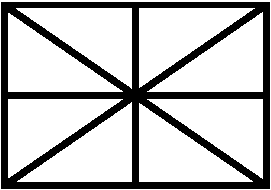
\includegraphics[width=0.9\columnwidth]{figure}}}
\caption{Figure captions are placed below the figure.}
\label{fig:example}
\end{figure}
Place tables/figures in text as close to the reference as possible
(see Figure~\ref{fig:example} and Table~\ref{tab:example}). They may extend
across both columns to a maximum width of 17.5cm (6.9").


% (end)

%%%%%%%%%%%%%%%%%%%%%%%%%%%%%%%%%%%%%%%%%%%%%%%%%%%%%%%%%%%%%%%%%%%%%%%%%%%%%%%%%%%%%%%%%%%

\section{Summary} % (fold)

Jamoma Foundation and DSP provide a flexible, user-extendable, runtime environment for creating and using audio and digital signal processing objects.  Due to its advanced use of dynamic binding and message-passing paradigm, the building blocks can be reconfigured at runtime without requiring re-compilation, but with the unit generators themselves compiled as C++ and performing block-processing we retain the performance of a compiled language.

The power of this runtime is demonstrated through the ability to compile objects for Max, Pd, AudioUnits, VST, etc.  The future includes Multicore.


% (end)

%%%%%%%%%%%%%%%%%%%%%%%%%%%%%%%%%%%%%%%%%%%%%%%%%%%%%%%%%%%%%%%%%%%%%%%%%%%%%%%%%%%%%%%%%%%

\section{Acknowledgements} % (fold)

Dave Watson, Joshua Kit Clayton, Théo Delahogue

% (end)

%%%%%%%%%%%%%%%%%%%%%%%%%%%%%%%%%%%%%%%%%%%%%%%%%%%%%%%%%%%%%%%%%%%%%%%%%%%%%%%%%%%%%%%%%%%

\bibliographystyle{IEEEtranS}
\bibliography{../../Shared/bibtex/Jamoma} % requires file template.bib

\end{document}
